\documentclass[acmtog]{acmart}

\usepackage{graphicx}
\usepackage{subfigure}
\usepackage{natbib}
\usepackage{listings}
\usepackage{bm}
\usepackage{amsmath}

\definecolor{blve}{rgb}{0.3372549, 0.61176471, 0.83921569}
\definecolor{gr33n}{rgb}{0.29019608, 0.7372549, 0.64705882}
\makeatletter
\lst@InstallKeywords k{class}{classstyle}\slshape{classstyle}{}ld
\makeatother
\lstset{language=C++,
	basicstyle=\ttfamily,
	keywordstyle=\color{blve}\ttfamily,
	stringstyle=\color{red}\ttfamily,
	commentstyle=\color{magenta}\ttfamily,
	morecomment=[l][\color{magenta}]{\#},
	classstyle = \bfseries\color{gr33n}, 
	tabsize=2
}
\lstset{basicstyle=\ttfamily}

% Title portion
\title{Final Project:\\ {Sparse Volume Visualization}} 

\author{Name:\quad  Wang Penghao, Zhou Shouchen  \\ student number:\ 2021533138,2021533042
\\email:wangph1@shanghaitech.edu.cn,zhoushch@shanghaitech.edu.cn}
\setlength{\headheight}{25pt}

% Document starts
\begin{document}
\maketitle

\vspace*{2 ex}

\section{Introduction}
In this project, we applied sparse volume rendering with advanced acceleration data structure in two methods: \\
\begin{itemize}
	\item serial CPU version
	\item parallel GPU opengl version
\end{itemize}
And following tasks are finished.\\
\begin{itemize}
\item load raw datas
\item volume rendering
\item acceleration structure
\item OpenGL
\end{itemize}
The following are the 3rd party library used in this project
\begin{itemize}
	\item Eigen3
	\item glad
	\item glfw
	\item glm
	\item imgui
\end{itemize}

\section{paper Introduction}
\subsection{Block Walking}
since the Volume rendering are calculating voxel by voxel, so we could speed up by using the method of block walking.\\
since we are doing the sparse volume rendering, so many of the voxels are useless,\\
to avoid doing so many times useless computing step by step in the empty voxel,\\
we can just skip that empty voxel, and go to the next voxel, by computing the interaction with the
ray and the small bounding box aabb of the voxel.\\
if the next voxel is still empty, it can continuous going to the next.\\

\subsection{Perfect Spatial Hashing}
since we are applying the sparse volume rendering, so many of the voxels are empty, without any useful imformations.\\
so using hashing could greatly save the space and time complexity.\\
And the paper provided some perfect spatial hashing methods.\\
For example, the hashing $h(p) = h_0(p) + \Phi [h_1(p)]$, the paper provided the method that $h_0,h_1$ are two simple hashing 
functions, and the function $\Phi$ is an offset table.\\
Written formally it is like mapping the point $p$ into:\\
$h(p) = h_0(p) + \Phi [h_1(p)]$\\
the pseduo formula is like $offset = tex(SOffset, h1) * oscale$ , where the paramaters have the computing method in the paper.\\
With the method of perfect Spatial hashing, we could greatly save the data scale, ignoring the large place of empty voxels.\\

\section{Implementation Details - CPU version}
The cpu version is based on the code from assignment 3 and assignment 4
\subsection{Load Raw Datas}
the raw datas store the imformation of the voxels.\\
the origin data are the type of uint8.\\
with the tranfering function, we could calculate the rgba information for each pixel.\\
And we could store the rgba information, calculate the position information of each pixel, which will be used in ray casting later.\\

\subsection{Volume Rendering}
We used ray casting for volume rendering.\\
We generate mulitiple rays per pixel for ray casting.\\
For each ray, we could calclate the interaction points with the big bounding box.\\
And the two interaction points' information $t\_in$ and $t\_out$ could be calculated.\\
Then we do ray casting from front-to-back from $t\_in$ to $t\_out$.\\
the two variables color and opacity can be calculated front-to-back through:\\\\
$C_{dst} = C_{dst} + (1 - \alpha_{dst}) \cdot C_{src}$\\
$\alpha_{dst} = \alpha_{dst} + (1 - \alpha_{dst}) \cdot \alpha_{src}$\\

since the point is not on exactly on voxel, so we could compute the point and their neighbor voxel's distance on
the three different directions(x,y,z axis),\\

with the usage of trilinear interpolation, we could compute the point's color and opacity information.\\


\subsection{Acceleration Structure}
When the opacity if close to 1(we chose $\alpha > 0.999$),
then we can stop the ray casting process to save time.\\
since the Volume is sparse, so the $t\_in, t\_out$ may calculate too much useless 
information if we just compute it with the huge $AABB$.\\
So we could use the bvh structure and block walking to get the closest $t\_in, t\_out$.\\
To improve more, the hashing method may be put into use.\\

\section{Implementation Details - GPU OpenGL version}
The GPU version is based on OpenGL, improved based on the code from assignment1.
\subsection{Load Data}
As for the raw data, we could use a OpenGL 3D texture to load data, simply read the data and bind it to the texture id is done. We also need to do cubic interpolation by using OpenGL texture's function. Which can be done easily. 
\subsection{Volume Render}
To realize a opengl volume renderer, we need to implement ray-casting in shader of OpenGL. 
Still we render a cube as the bounding box.\\
Firstly, we still need VAO, VBO, EBO to render a simple cube. After doing so, we need to calculate the ray generate from camera. This is hard to do on glsl Shader by using coordinate transformation, therefore, we implement a new way to do so. 
We need to find the entry point and exit point for the cube with the ray. We could calculate by using ray and AABB intersect. However, this is hard to do as we need to apply coordinate transformation for ray. As for the entry point, we can get it simply from the vertex shader, which is the gl. As for the exit point, opengl has a new feature called "cull face", therefore, we can only render for back faces of the cube. Then how we get the depth? We can create a depth buffer and in the render loop, we could render depth to this buffer, then link it to a 2D texture and transform it to GPU in fragment shader.
\subsection{RayCasting}
After get the entry point and the exit point, we could create a ray, and then we need to find the color for this ray, we can read the raw data and store it as a 3D texture, then link it with shader. After that we could make raycasting by make loop in fragment shader by addinig unit vector to the ray vector. Then we can get the color by using texture for each sample point, then send it to transfer function to get RGBA. As this texture uv search is on the gpu, which is fast enough, the result is real-time. Then make alpha-blending to get the result color. 
\subsection{Interactive and FPS}
We implement simple interactive by moving camera and view direction with keyboard and mouse, which came from assignment1. 
To calculate FPS, we calculate time for rendering each frame. Then we use imgui to show it on the screen. As glfw has the limit to sync the display's refresh rate, the calculate is much smaller then the actually rate. On 75hz display, our gpu version runs about 70-80fps. With a higher refresh rate, we will get a higher fps. 
 

\section{result}
\begin{itemize}
	\item the first image is rendered on cpu with the original volume rendering method.\\
	\item the last three images are with the method of using OpenGL, they are using the diffenert datasets.\\
\end{itemize}


\begin{figure}[h]
	\centering
	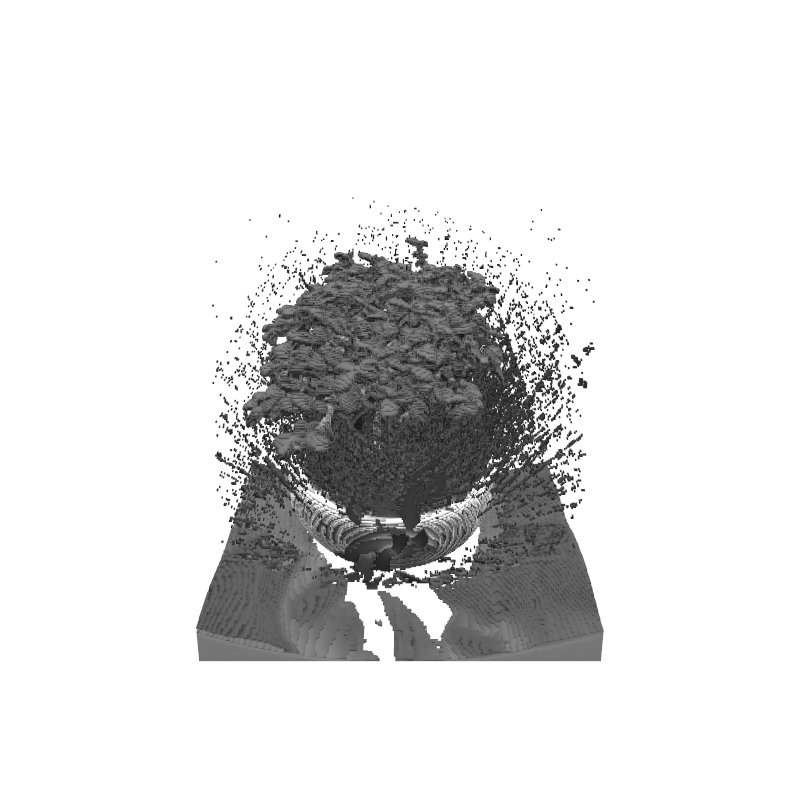
\includegraphics[width=4cm,height=5cm]{result_cpu}
	\caption{cpu-bonsai}
\end{figure}

\begin{figure}[h]
	\centering
	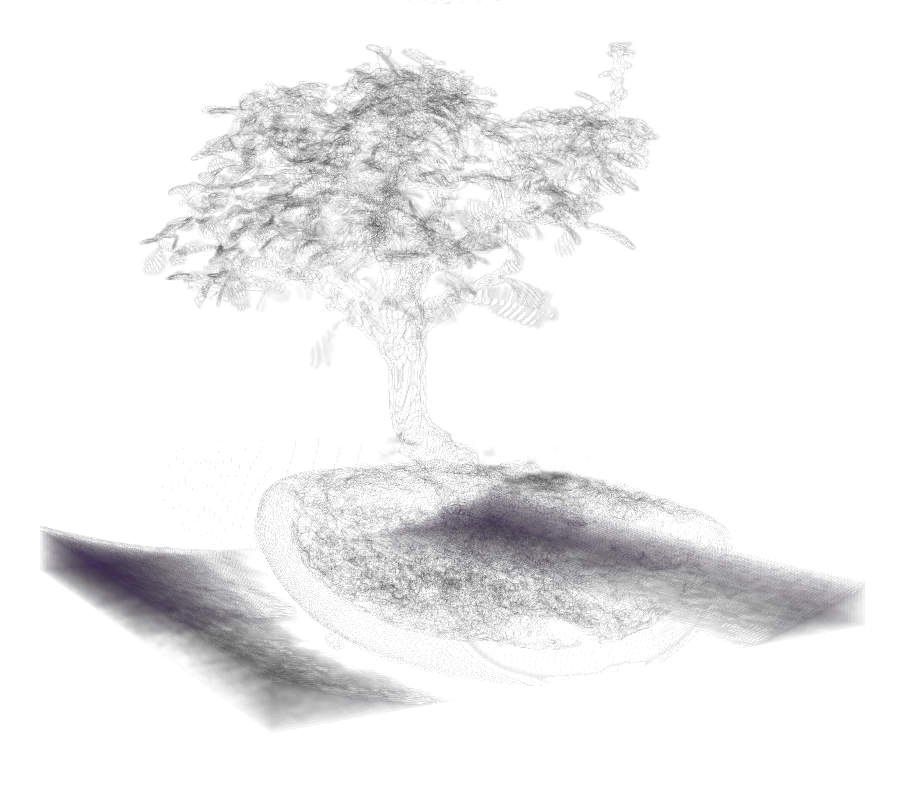
\includegraphics[width=4cm,height=5cm]{gpu_bonsai}
	\caption{gpu-bonsai}
\end{figure}

\begin{figure}[h]
	\centering
	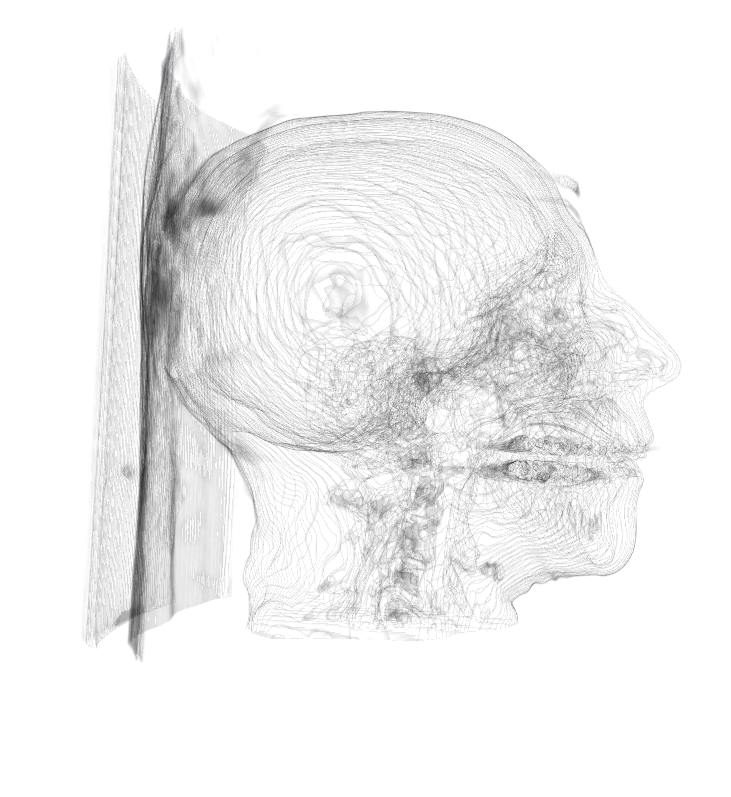
\includegraphics[width=4cm,height=5cm]{gpu_head}
	\caption{gpu-head}
\end{figure}

\begin{figure}[h]
	\centering
	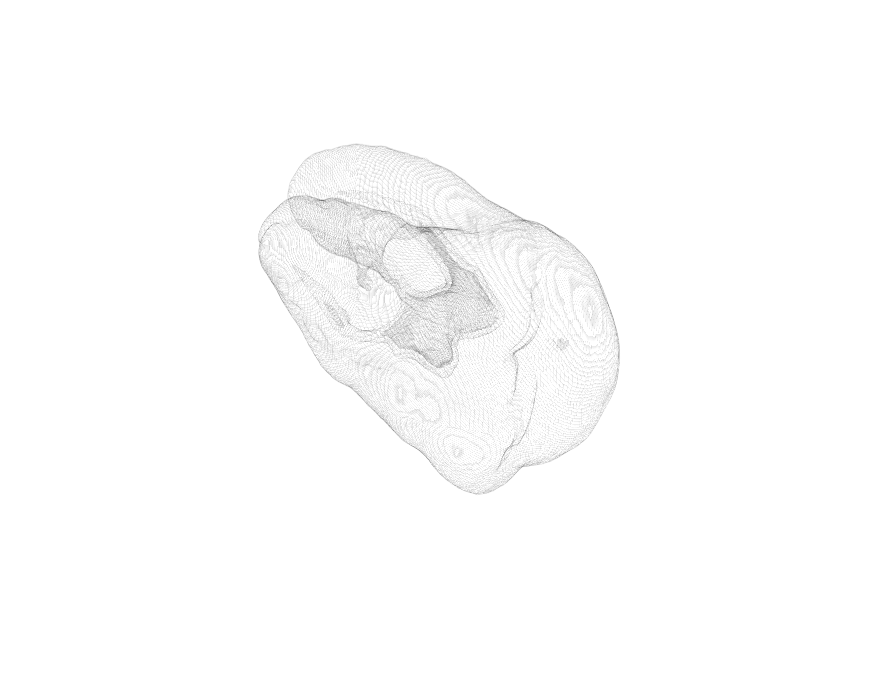
\includegraphics[width=4cm,height=5cm]{gpu_tooth}
	\caption{gpu-tooth}
\end{figure}
.
\\
\end{document}
